\documentclass[10pt,twocolumn,letterpaper]{article}

\usepackage[pagenumbers]{cvpr} % To force page numbers, e.g. for an arXiv version

\usepackage{graphicx}
\usepackage{amsmath}
\usepackage{amssymb}
\usepackage{booktabs}
\usepackage[acronym]{glossaries}

\usepackage[pagebackref,breaklinks,colorlinks]{hyperref}

\usepackage[capitalize]{cleveref}
\crefname{section}{Sec.}{Secs.}
\Crefname{section}{Section}{Sections}
\Crefname{table}{Table}{Tables}
\crefname{table}{Tab.}{Tabs.}

\def\cvprPaperID{*****}
\def\confName{CVPR}
\def\confYear{2022}

\graphicspath{ {./figures/} }
\DeclareGraphicsExtensions{.pdf,.jpg,.png}

\newacronym{svm}{SVM}{Support Vector Machine}
\newacronym{cnn}{CNN}{Convolutional Neural Network}
\newacronym{pca}{PCA}{Principal Component Analysis}


\begin{document}

\title{Star Tracker without a Star Database}

\author{Stephen Scott\\
McMaster University\\
1280 Main St W, Hamilton, ON L8S 4L8\\
{\tt\small scotts24@mcmaster.ca}
}
\maketitle

%%%%%%%%% ABSTRACT
\begin{abstract}
   The ABSTRACT is to be in fully justified italicized text, at the top of the left-hand column, below the author and affiliation information.
   Use the word ``Abstract'' as the title, in 12-point Times, boldface type, centered relative to the column, initially capitalized.
   The abstract is to be in 10-point, single-spaced type.
   Leave two blank lines after the Abstract, then begin the main text.
   Look at previous CVPR abstracts to get a feel for style and length.
\end{abstract}

%%%%%%%%% BODY TEXT
\section{Introduction}
\label{sec:intro}

Spacecraft attitude determination is the process by which a satellite uses sensors to estimate its orientation and is important to the satellite control problem because it provides a means for the satellite to adjust its trajectory with respect to a reference vector.

\section{Related Work}
\label{sec:related}

\section{Proposed Method}
\label{sec:method}

\begin{figure}[h]
  \centering
   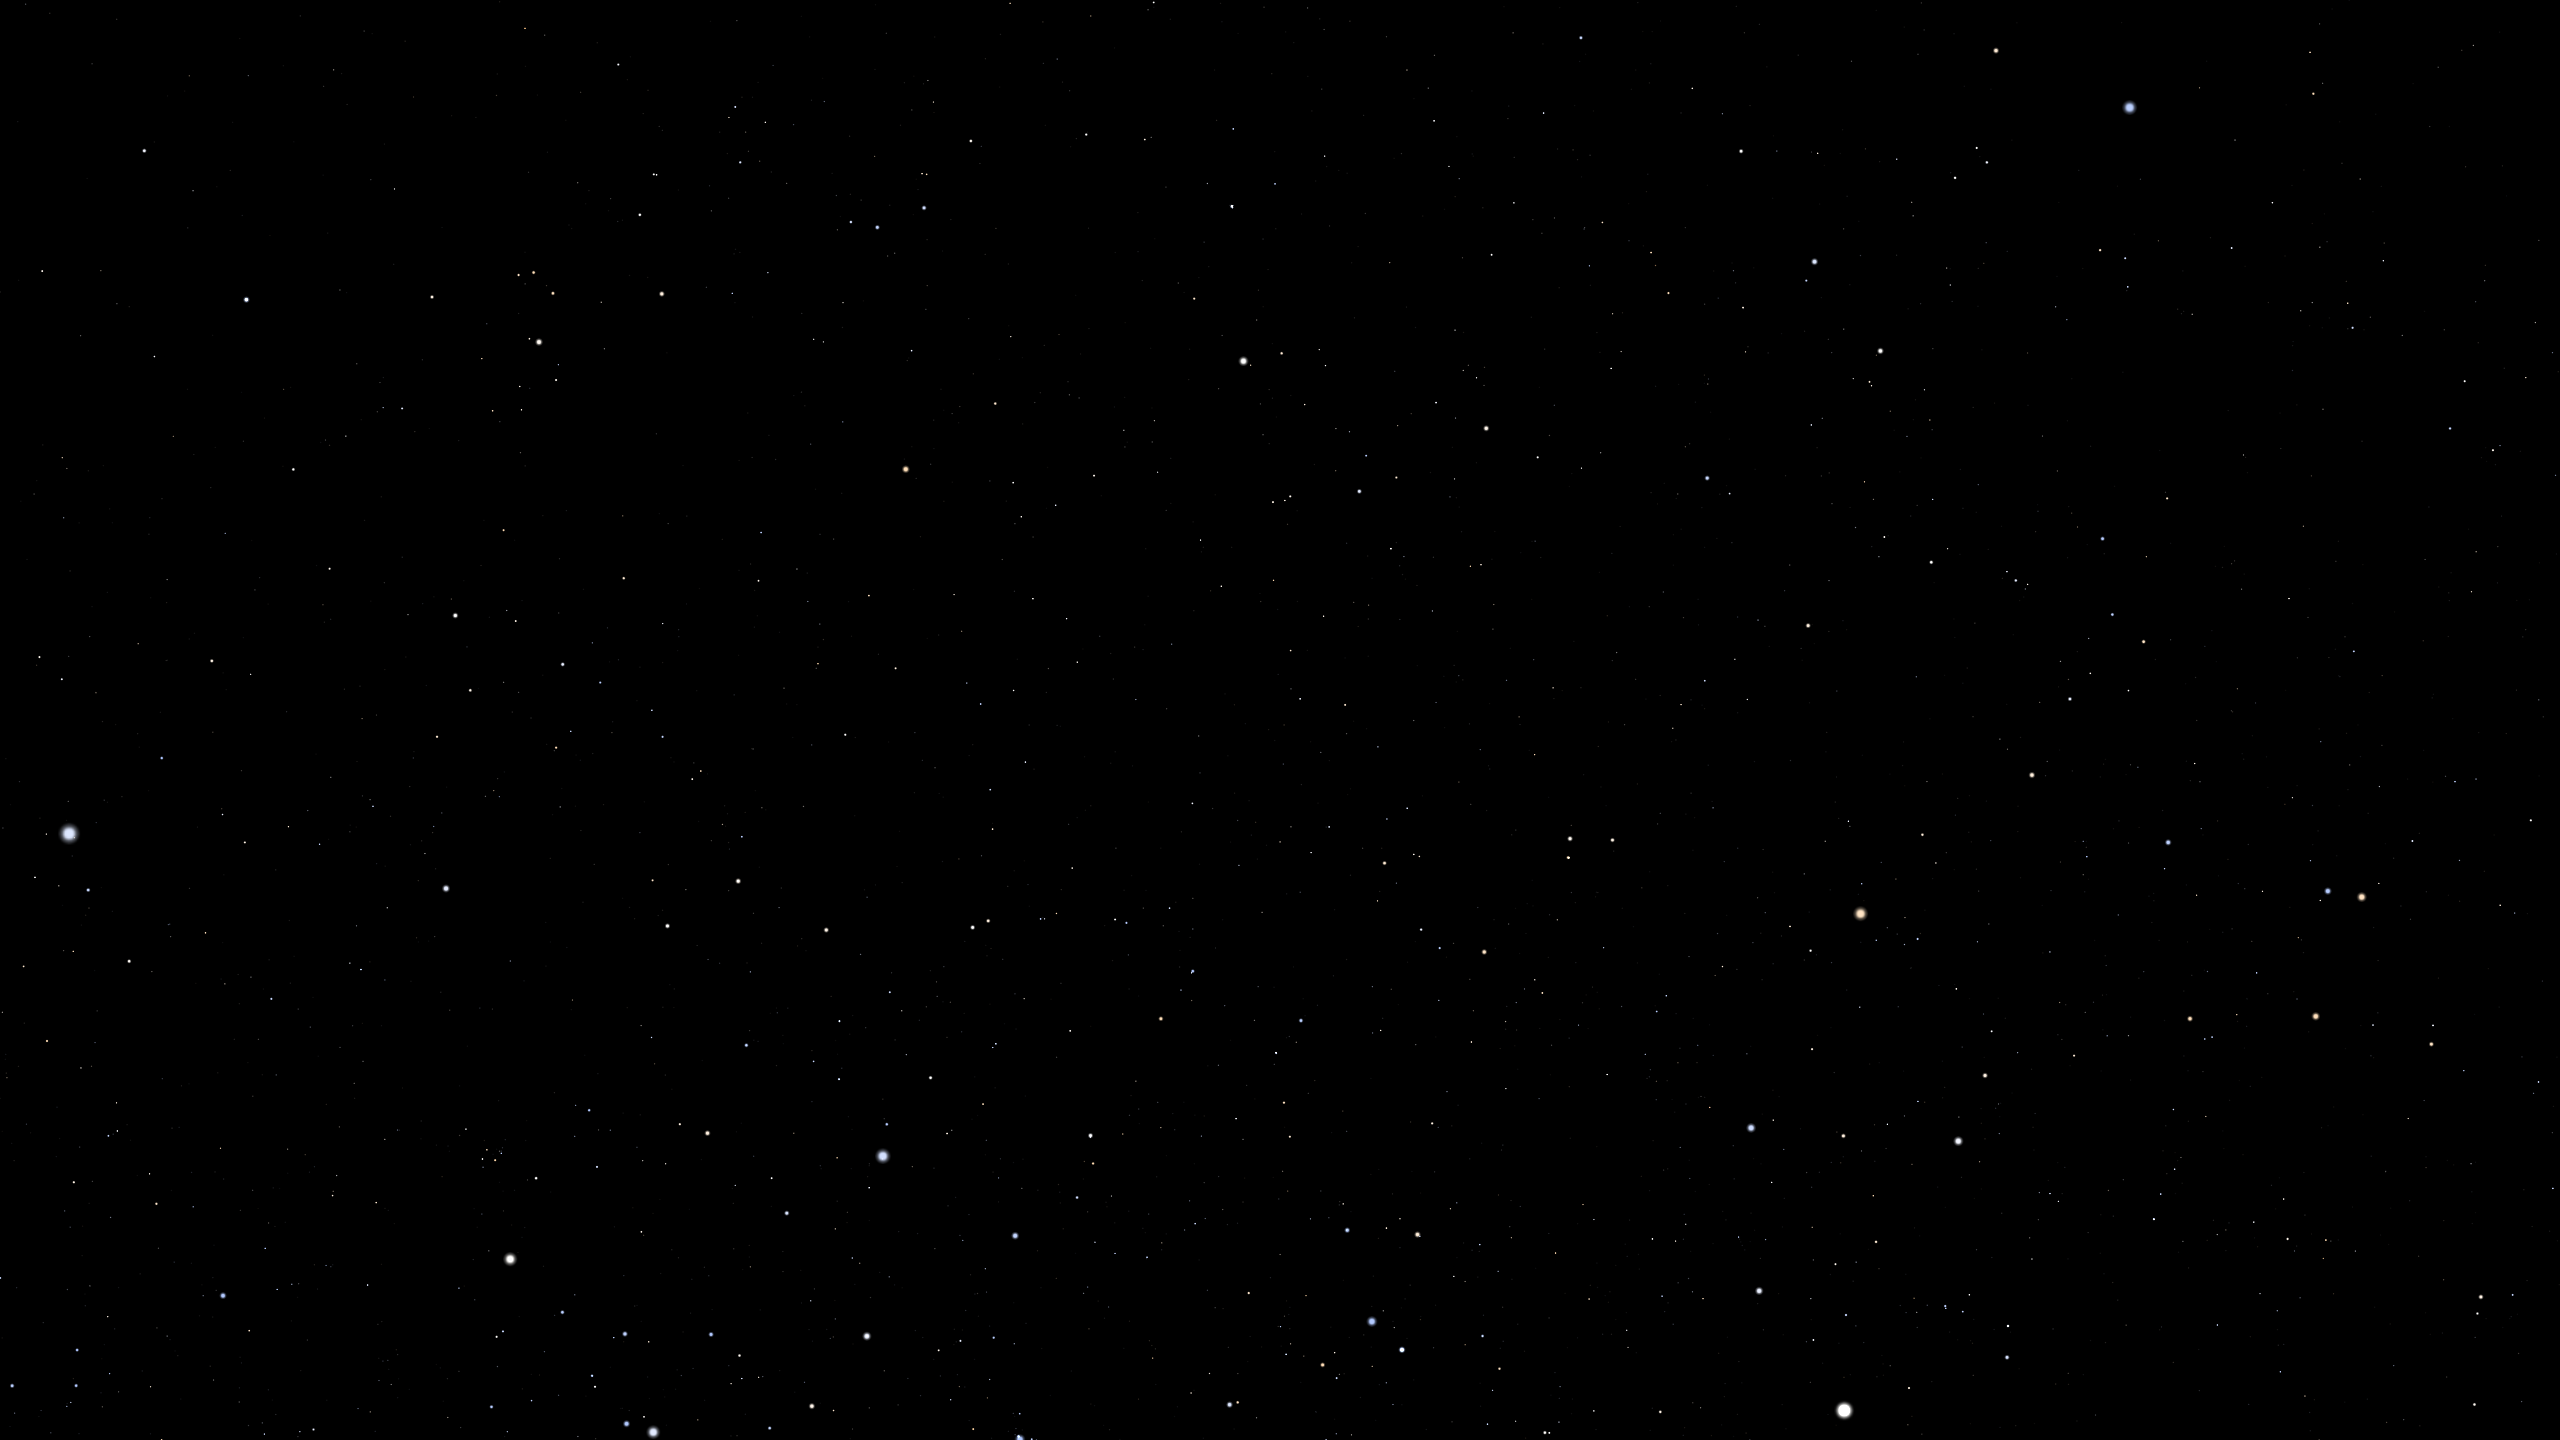
\includegraphics[width=0.9\linewidth]{stars_000}
   \caption{Example image from the star image dataset}
   \label{fig:star_img}
\end{figure}

\begin{figure}[h]
  \centering
   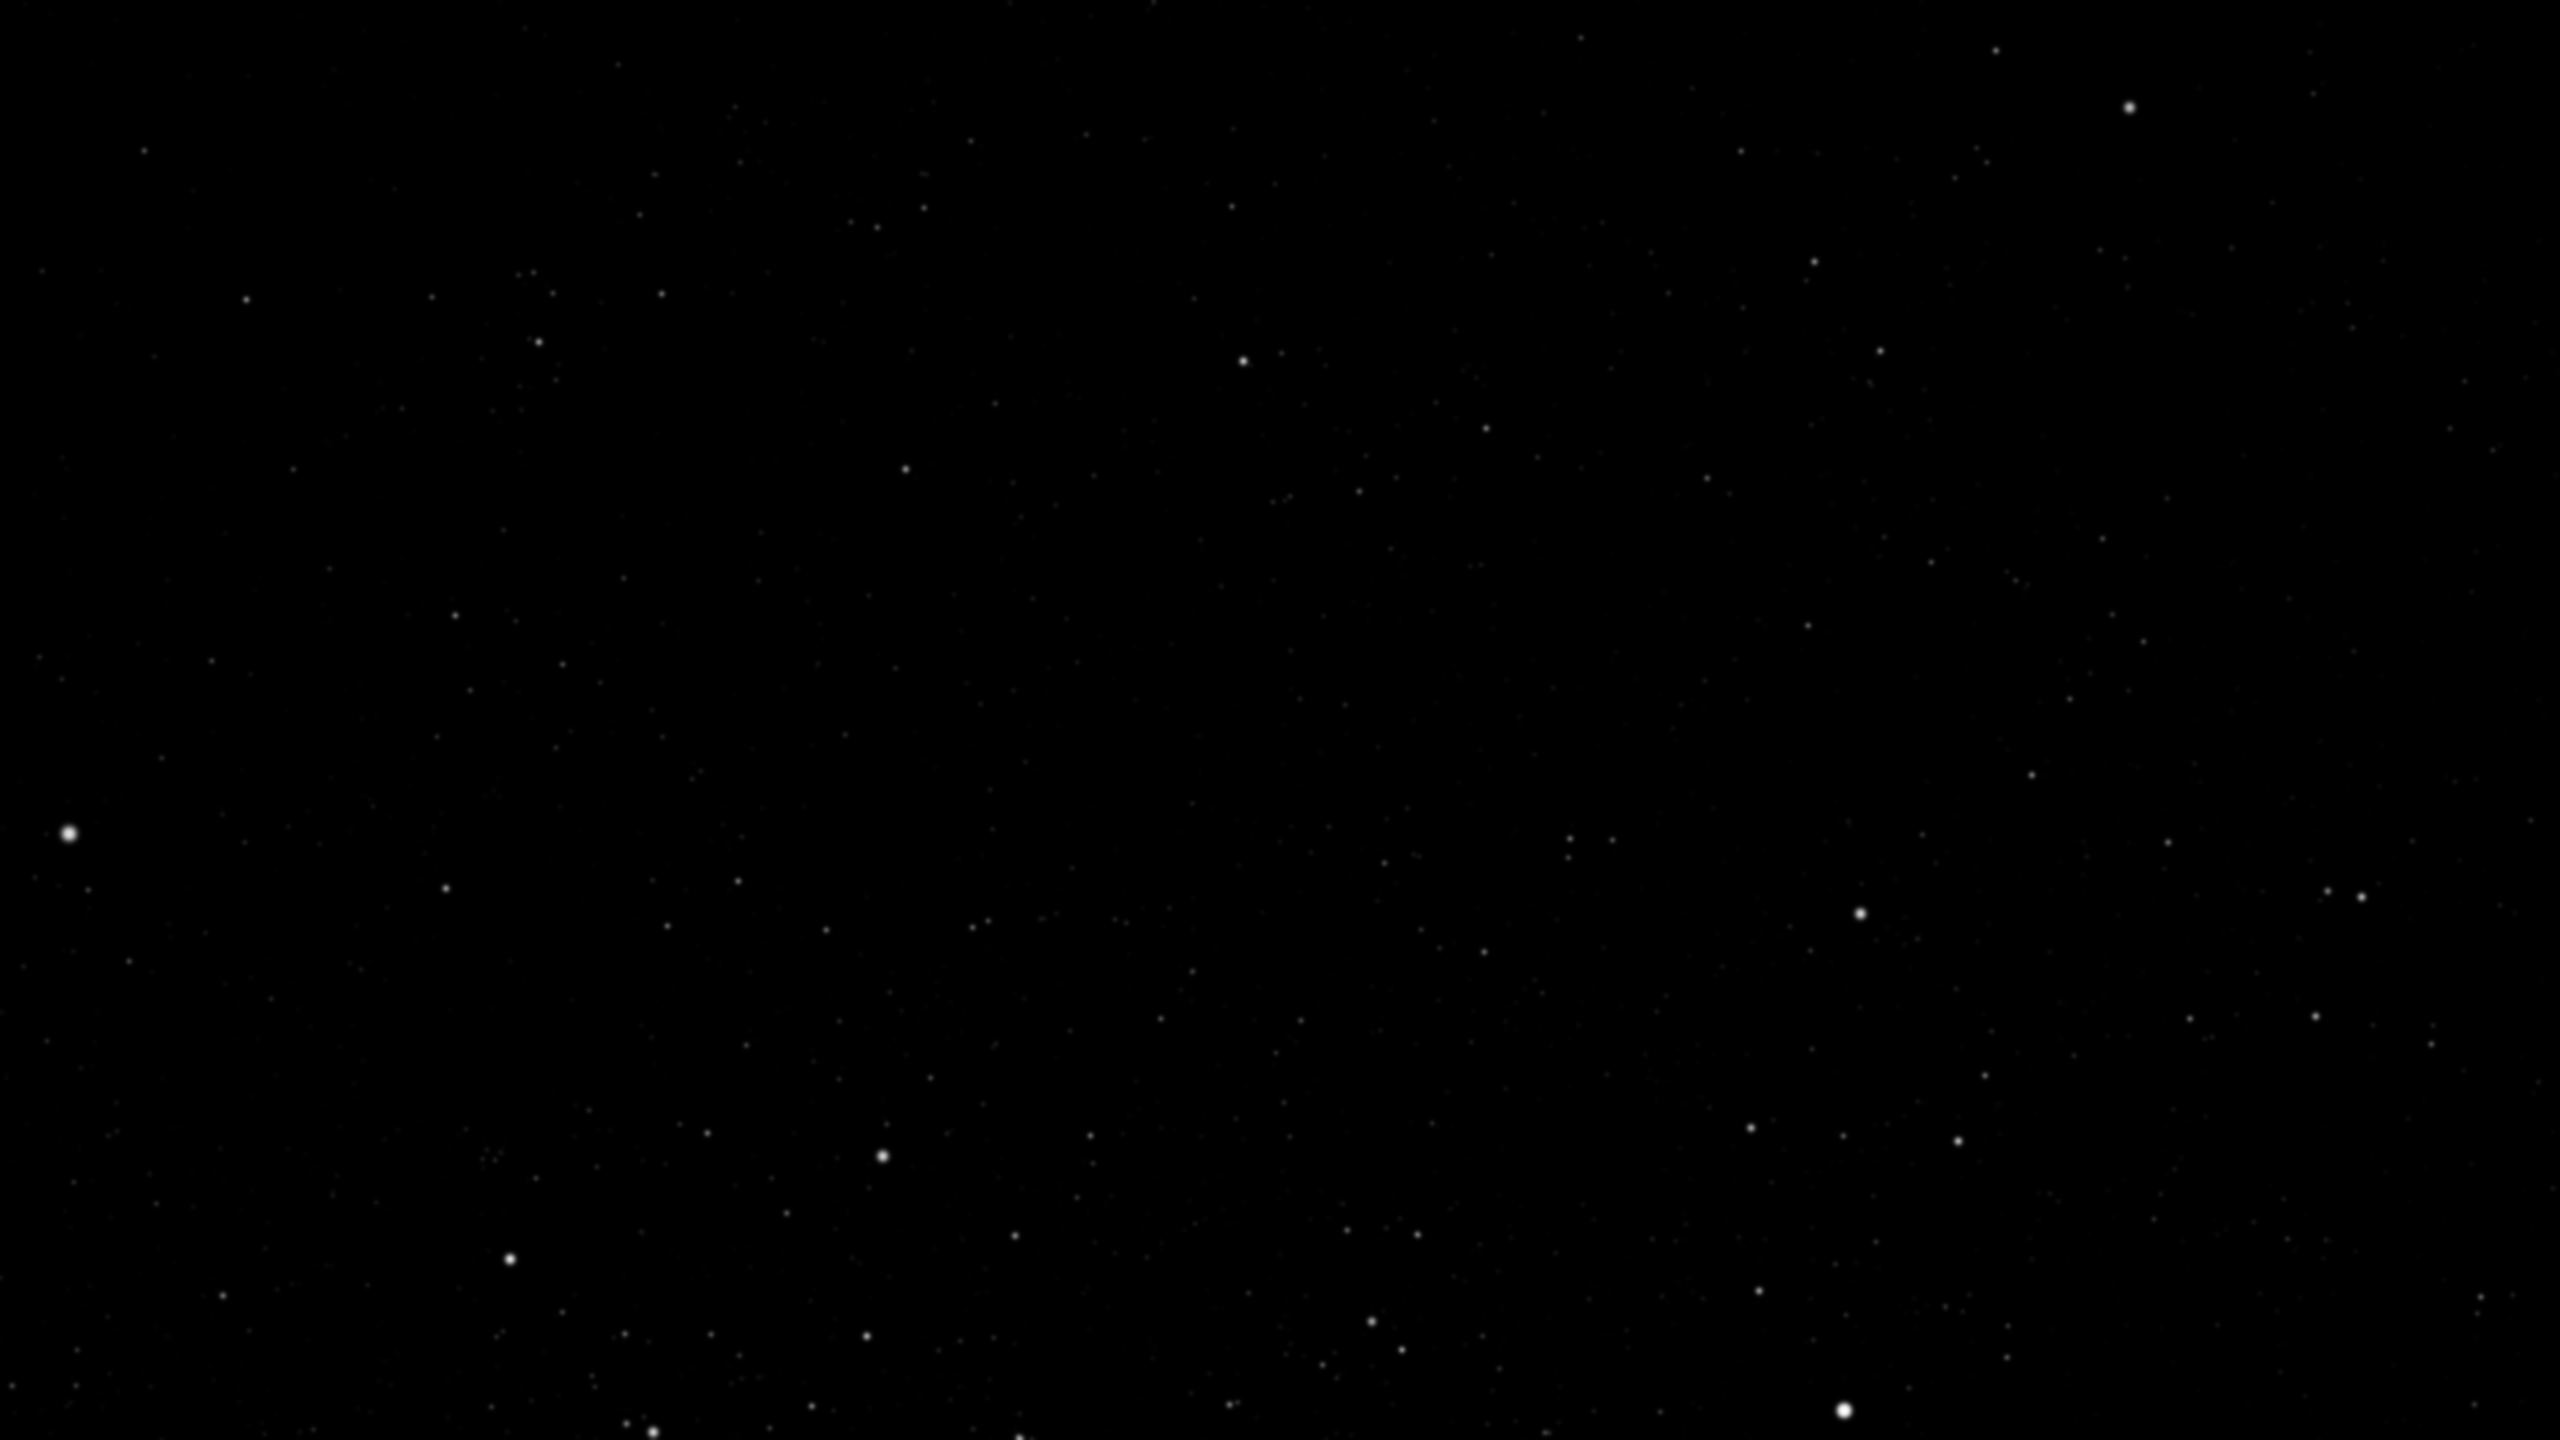
\includegraphics[width=0.9\linewidth]{gauss}
   \caption{Gaussian blur applied to star image}
   \label{fig:star_gauss}
\end{figure}

\begin{figure}[h]
  \centering
   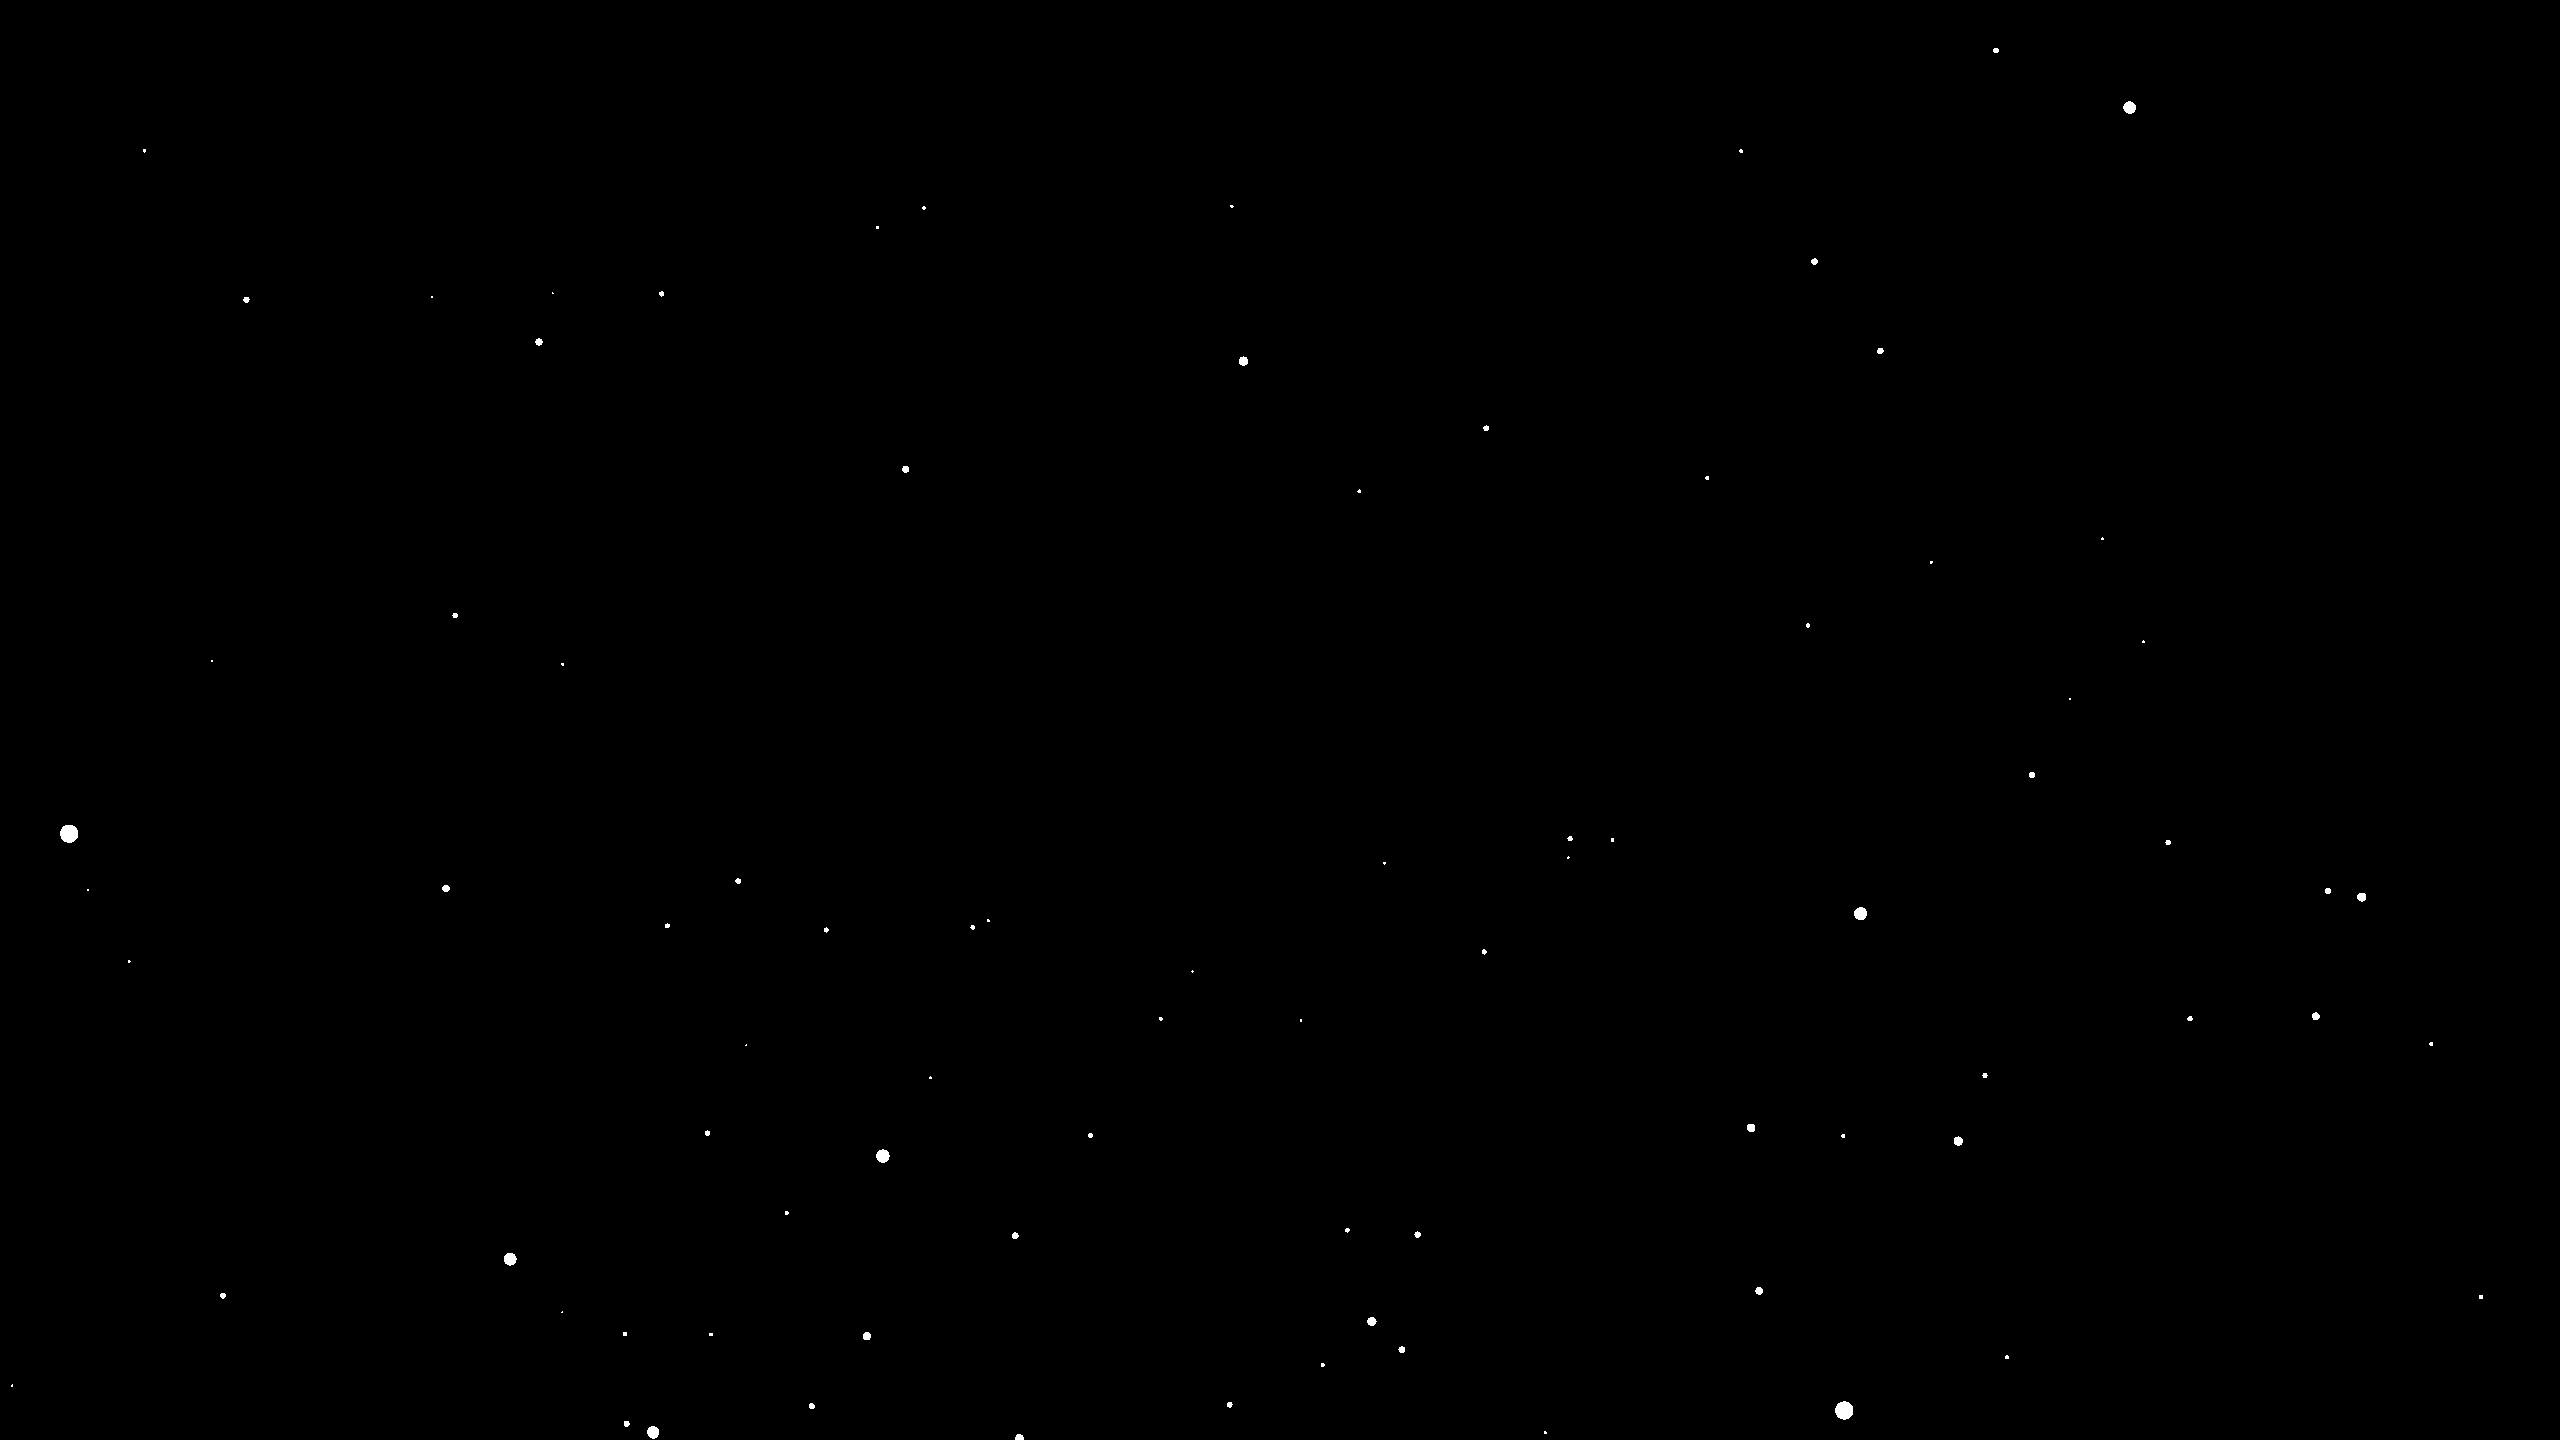
\includegraphics[width=0.9\linewidth]{binary}
   \caption{Result of binarizing the Gaussian blurred image}
   \label{fig:star_binary}
\end{figure}

\begin{figure}[h]
  \centering
   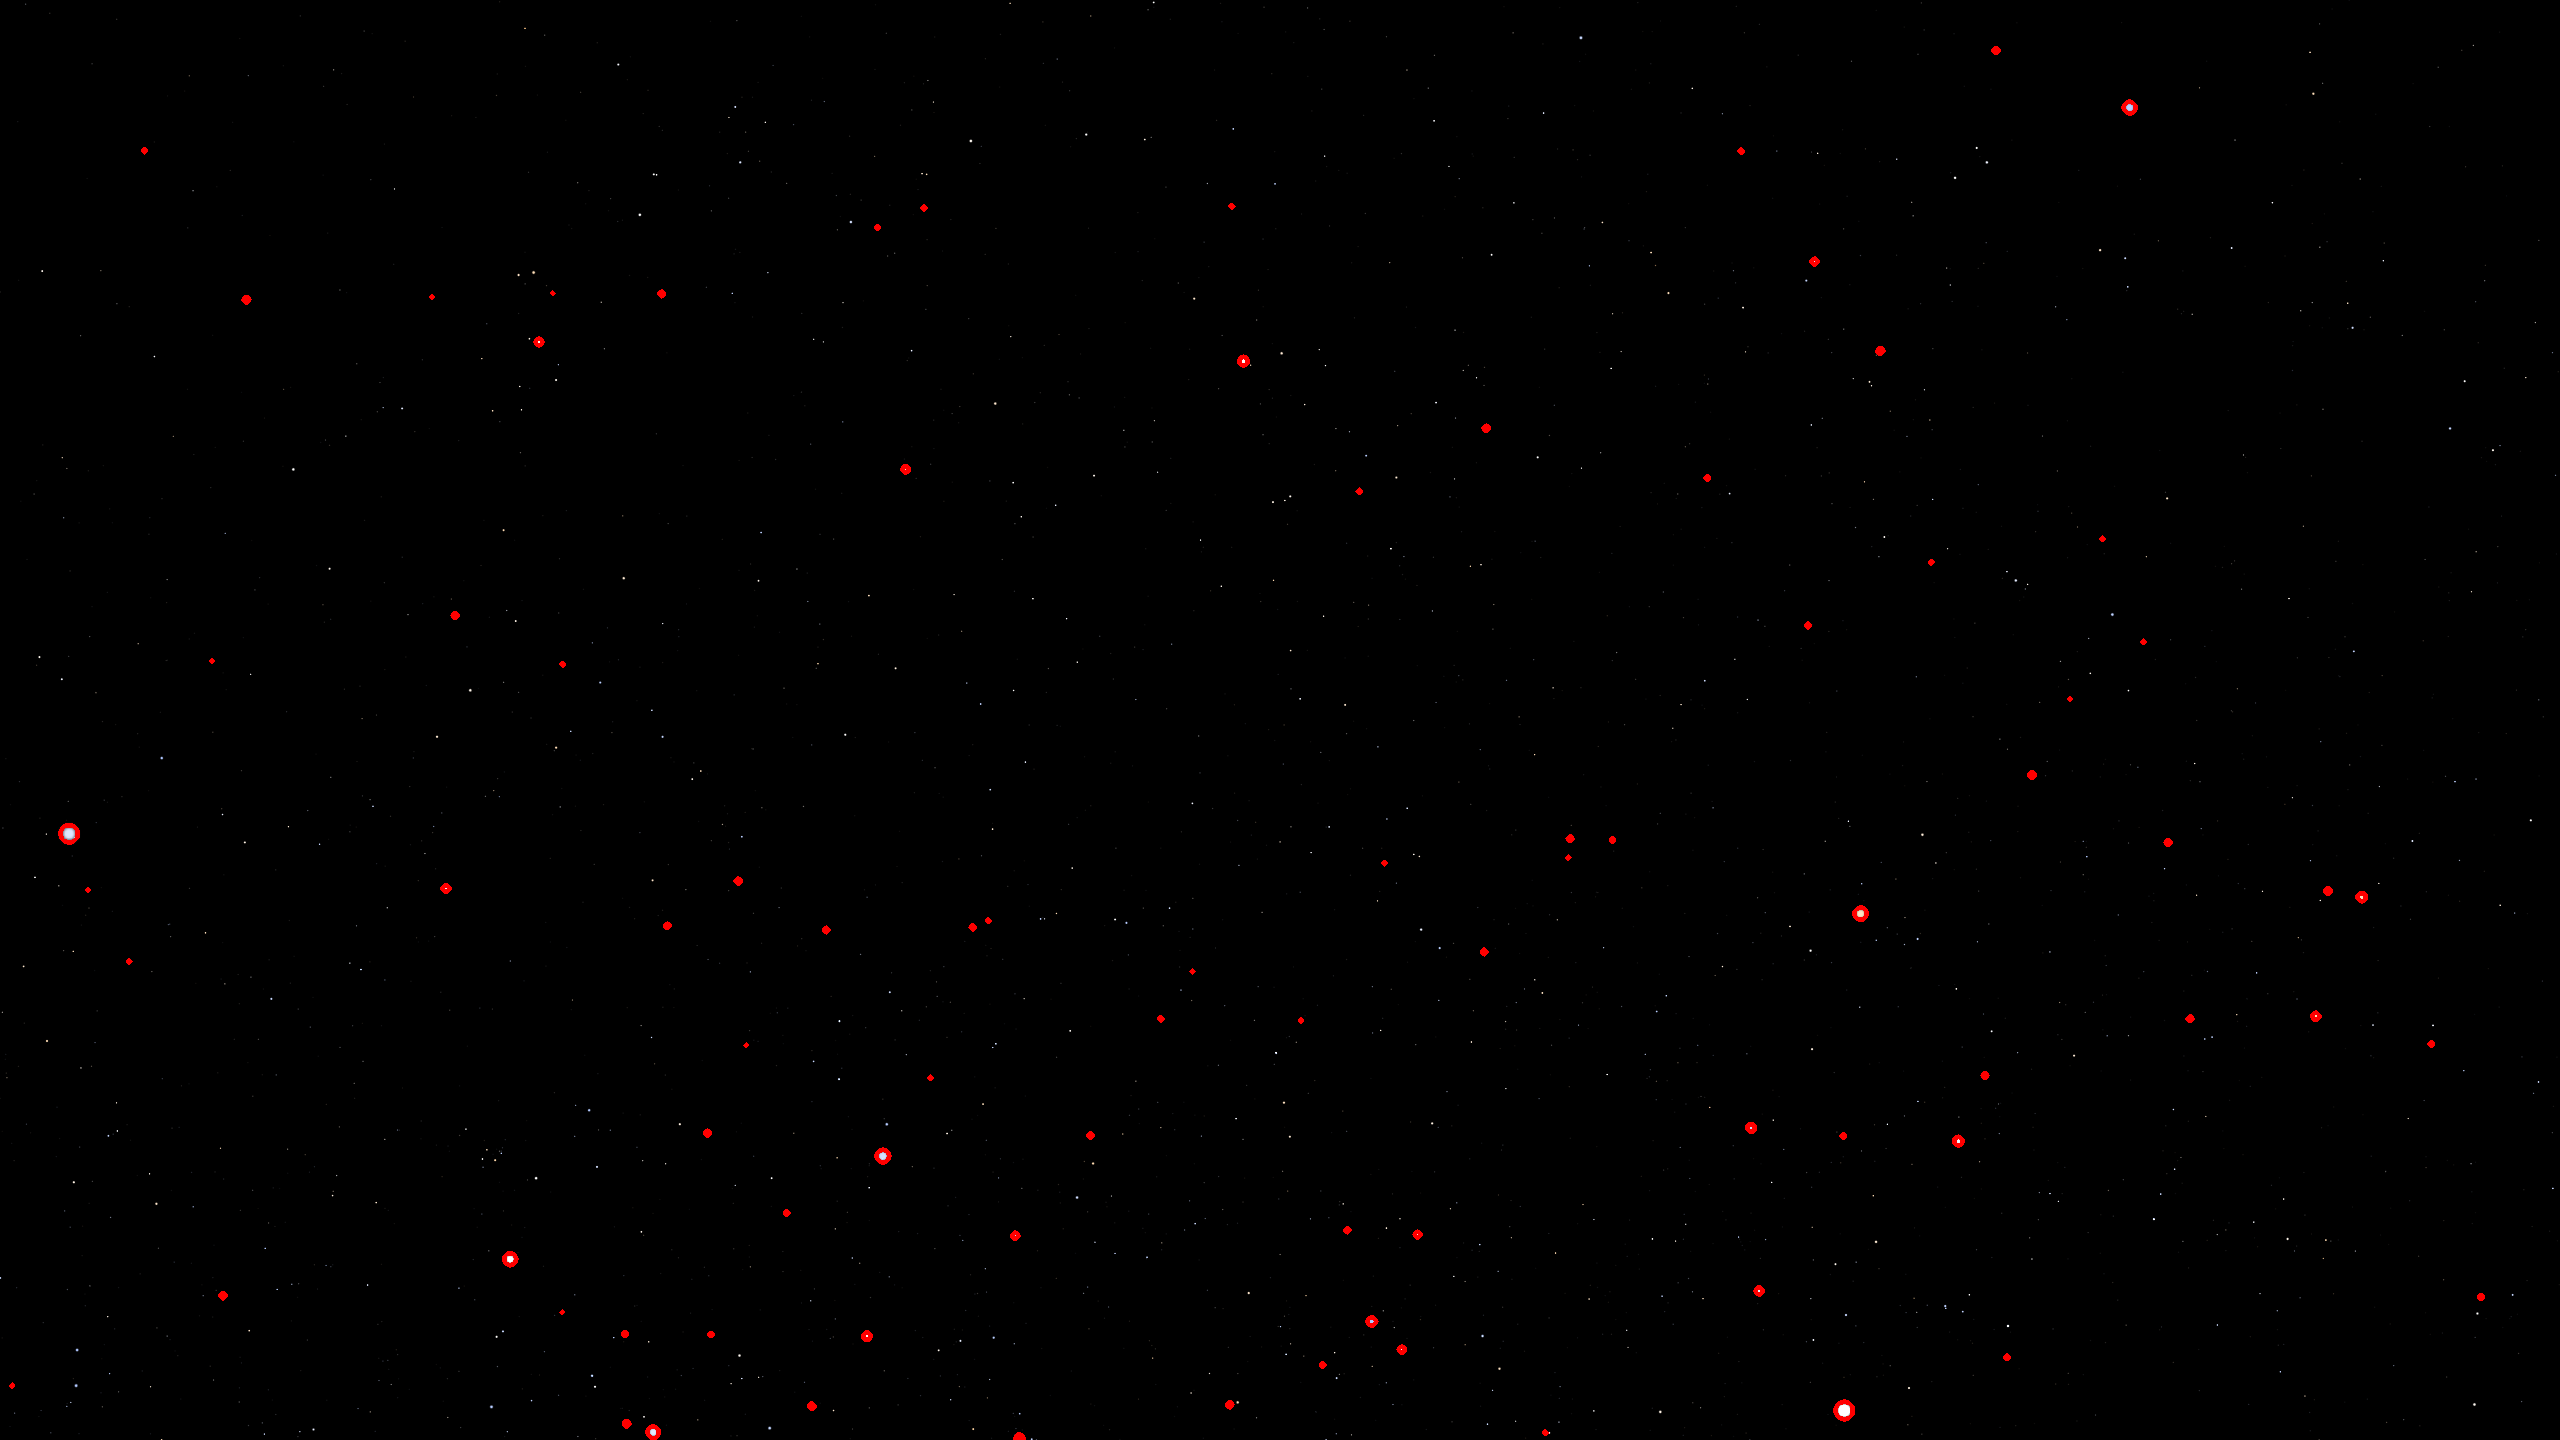
\includegraphics[width=0.9\linewidth]{all_contours}
   \caption{Result of locating global contours}
   \label{fig:star_contours}
\end{figure}

\begin{figure}[h]
  \centering
   
\includegraphics[width=0.9\linewidth]{mask}
   \caption{Circular mask around largest detected contour}
   \label{fig:star_mask}
\end{figure}

\begin{figure}[h]
  \centering
   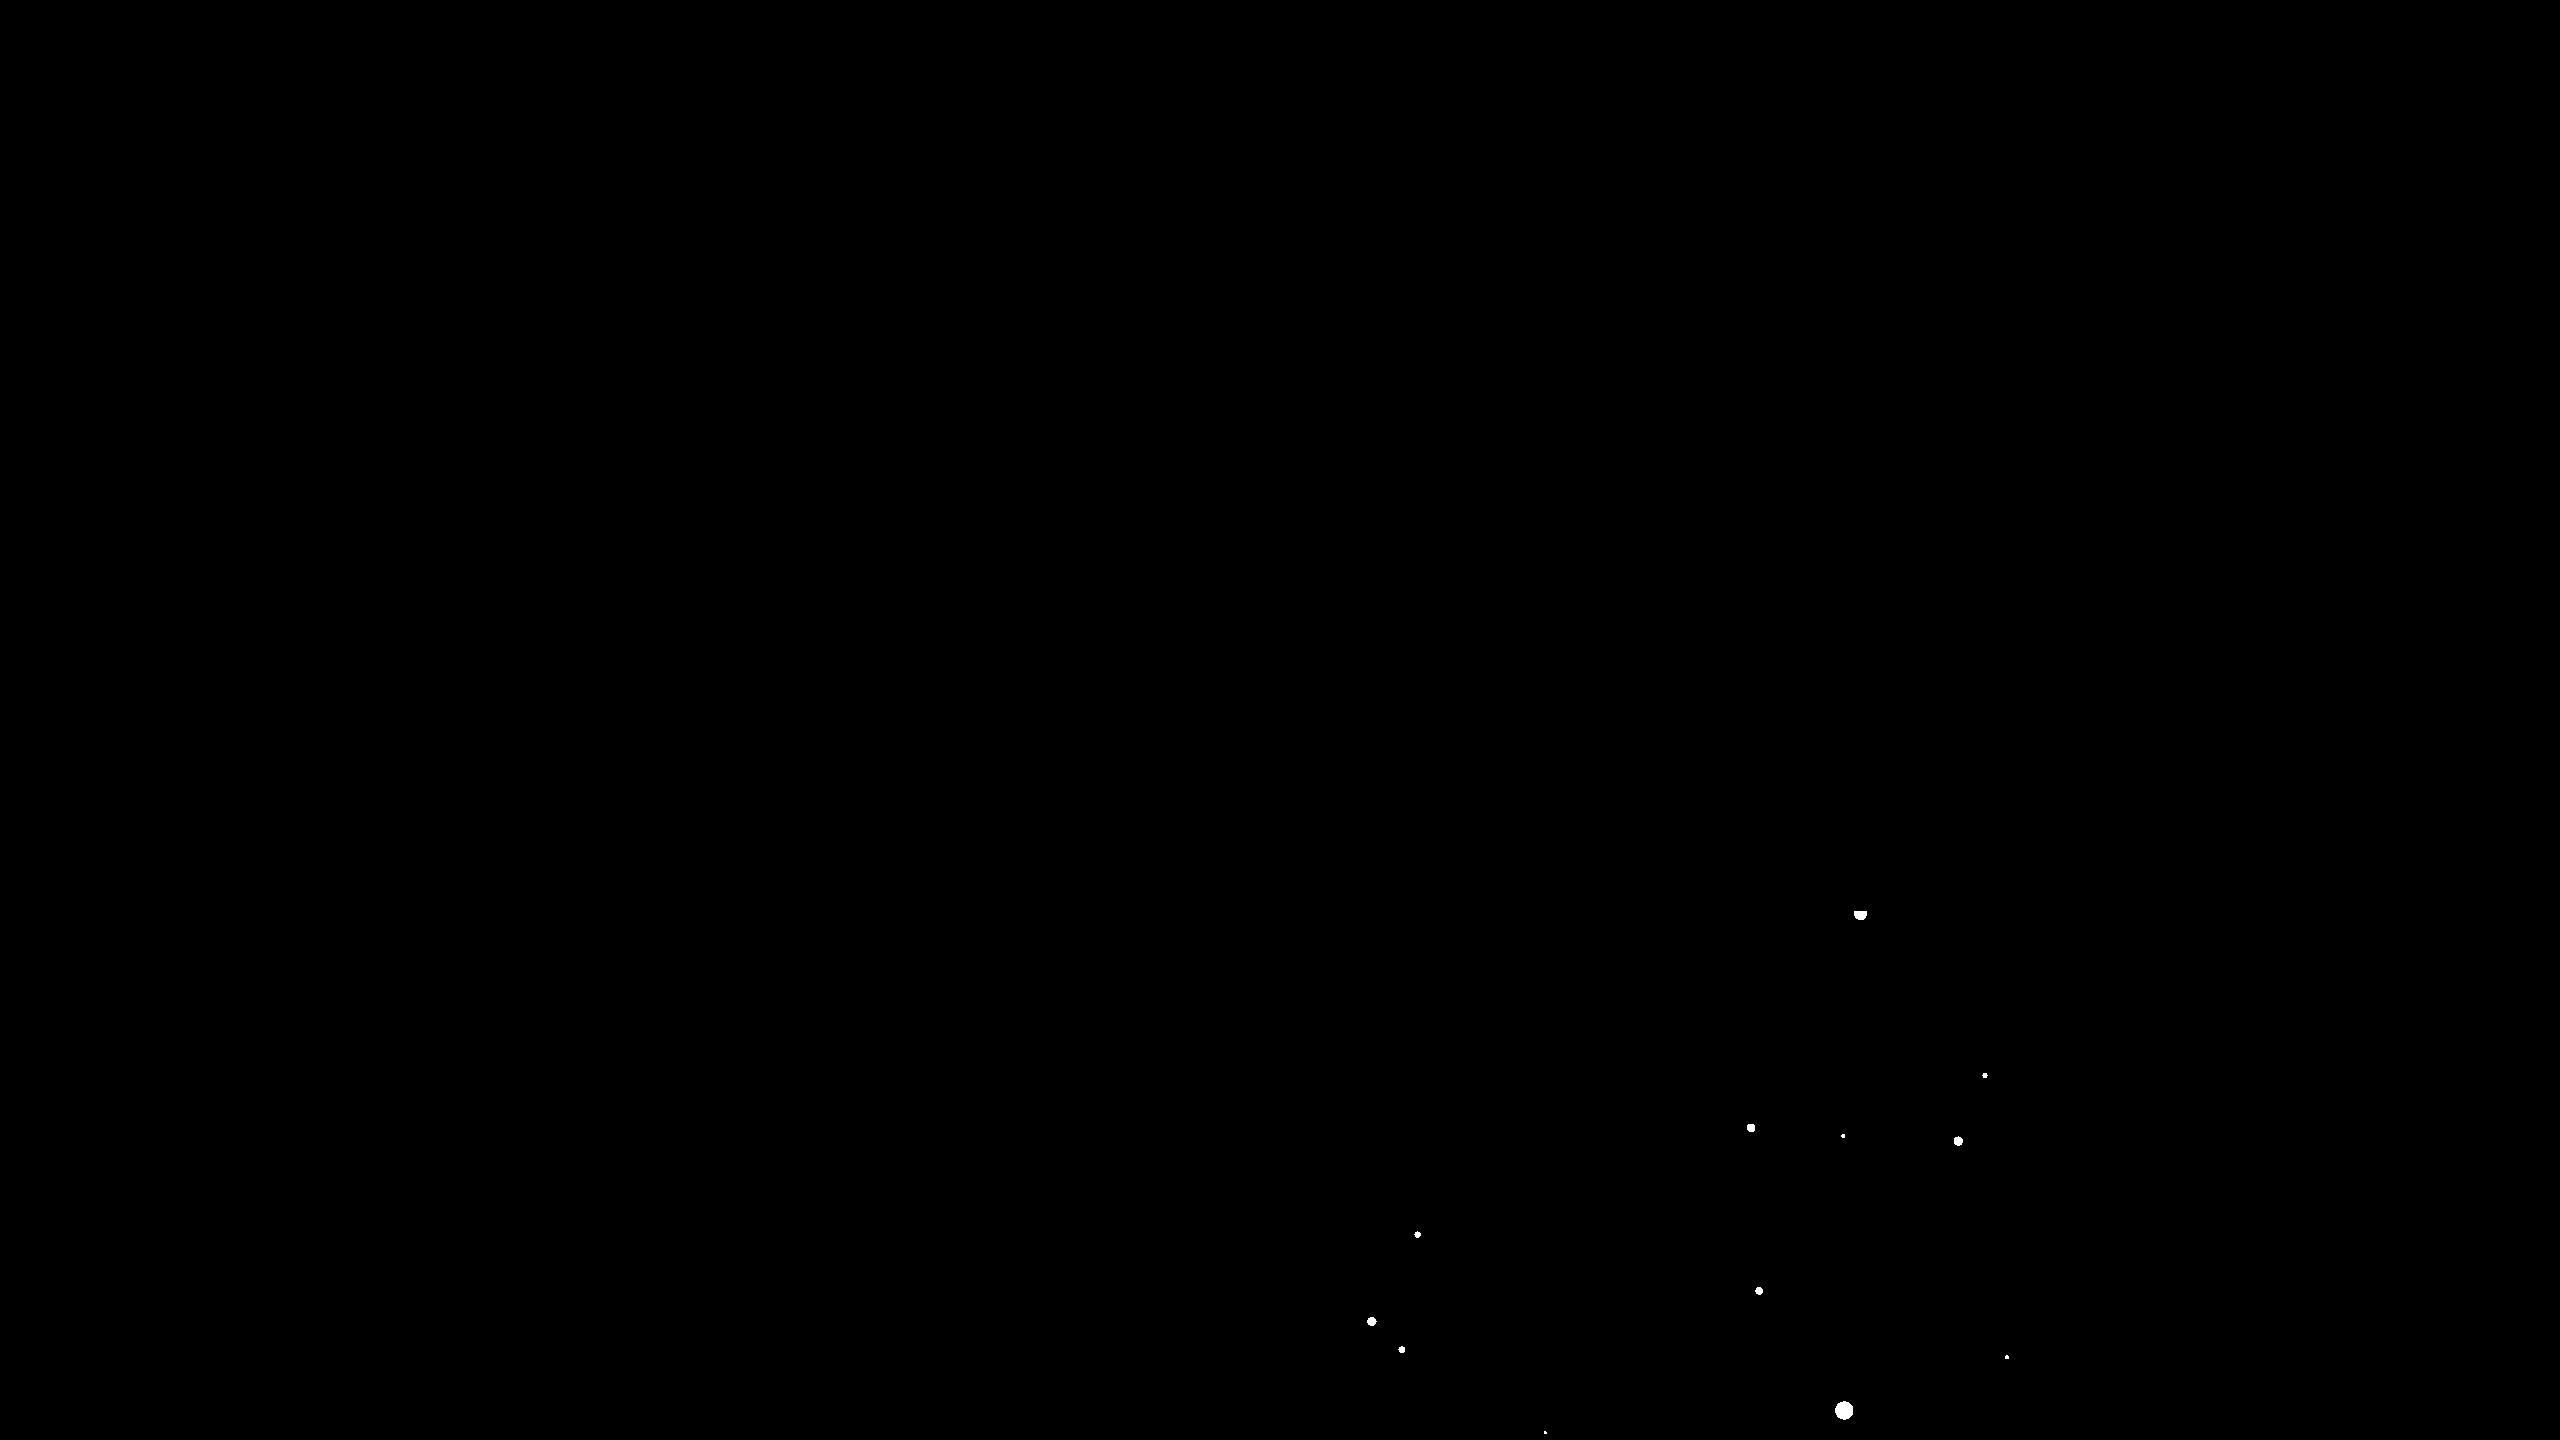
\includegraphics[width=0.9\linewidth]{masked}
   \caption{Result of applying the mask to the binarized image}
   \label{fig:star_masked}
\end{figure}

\begin{figure}[h]
  \centering
   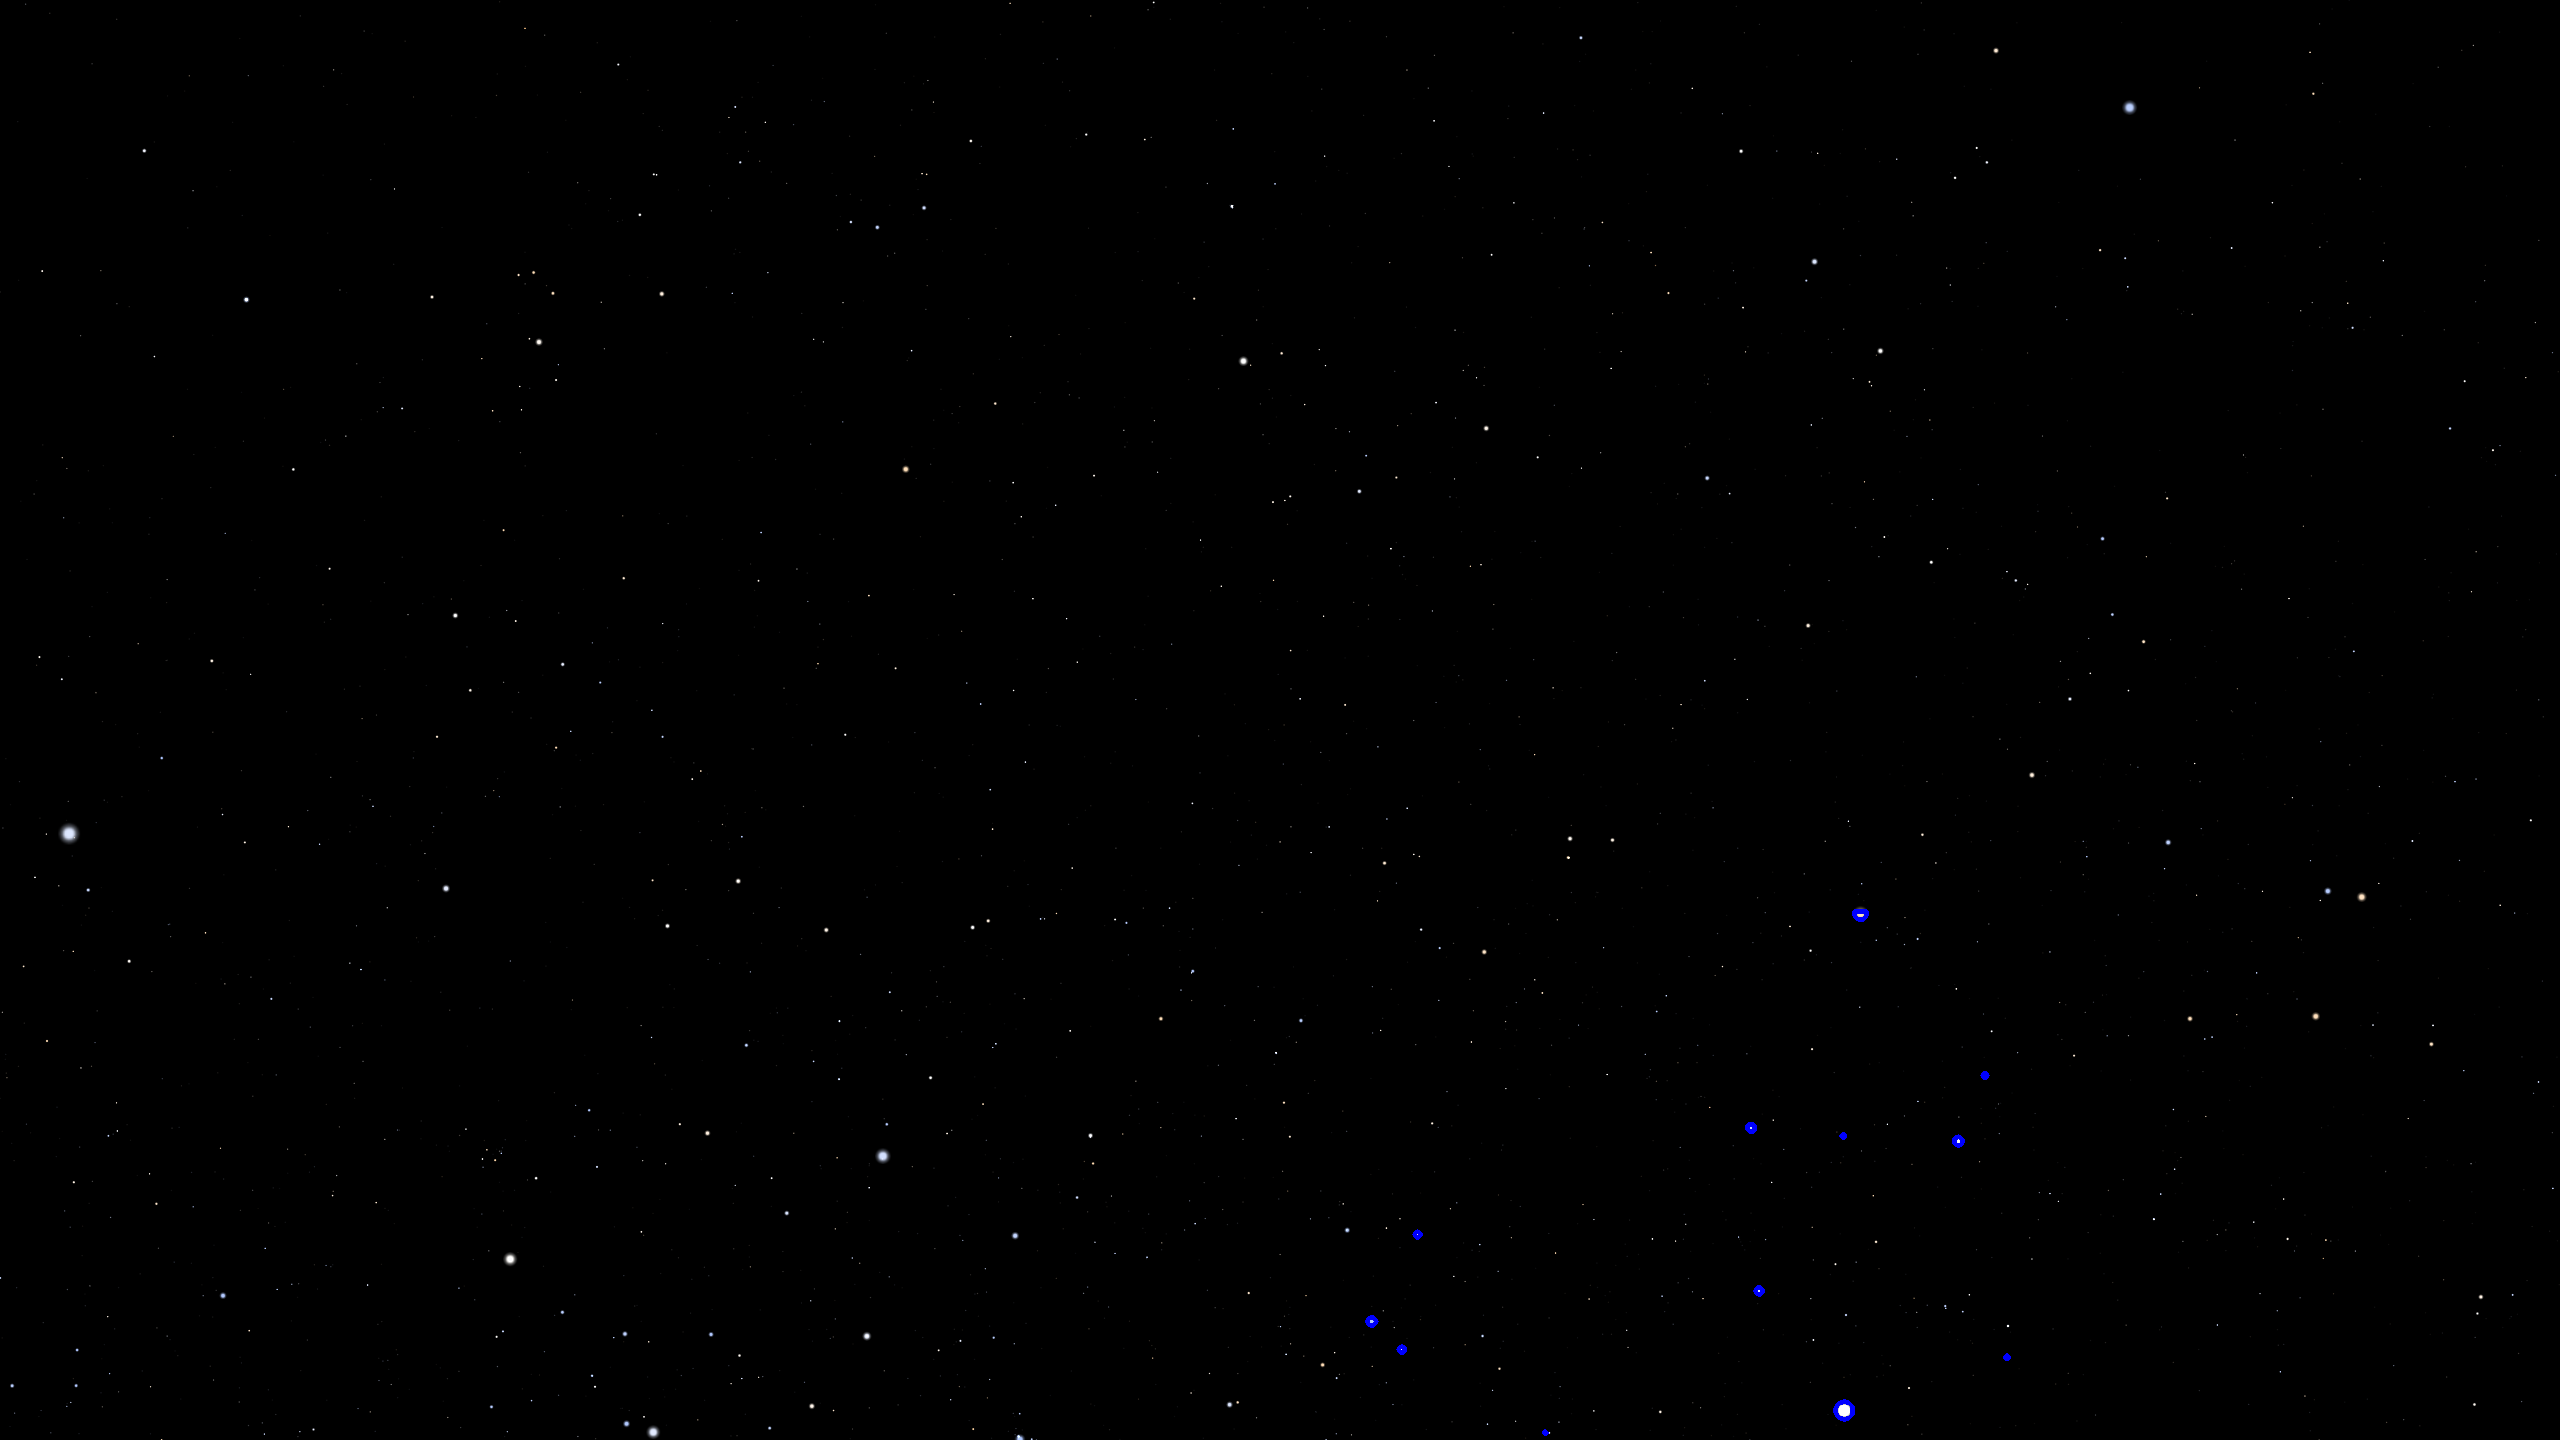
\includegraphics[width=0.9\linewidth]{local_contours}
   \caption{Result of locating contours in the masked region}
   \label{fig:star_local_contours}
\end{figure}

\begin{figure}[h]
  \centering
   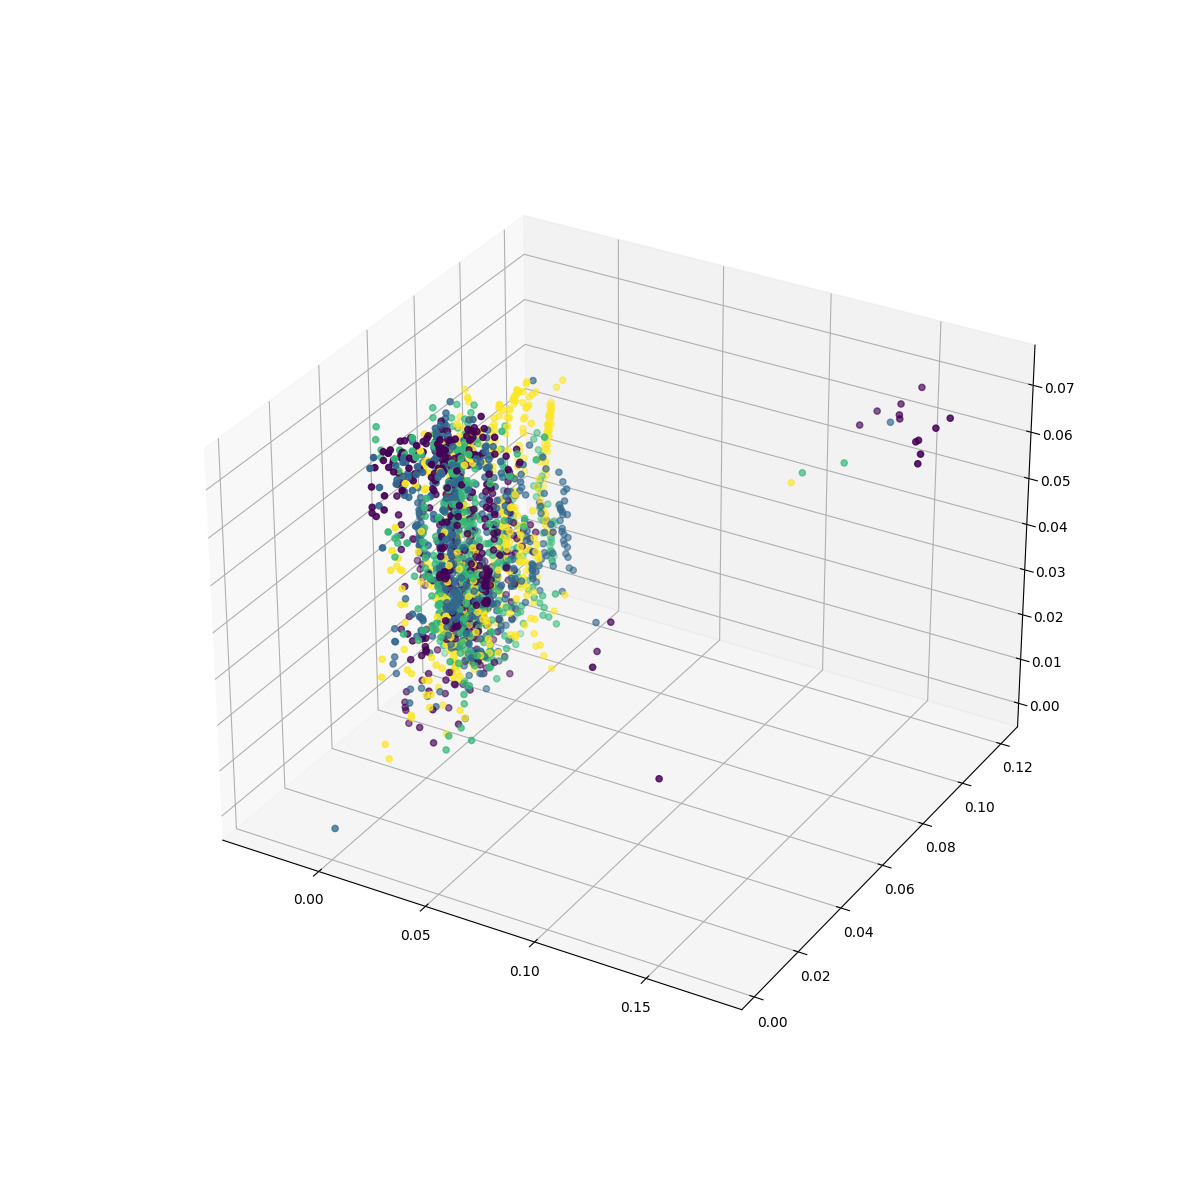
\includegraphics[width=0.9\linewidth]{pca}
   \caption{\acrlong{pca} applied to the normalized training data}
   \label{fig:pca}
\end{figure}

\section{Alternate Method}
\label{sec:alt_method}

\begin{figure}[h]
  \centering
   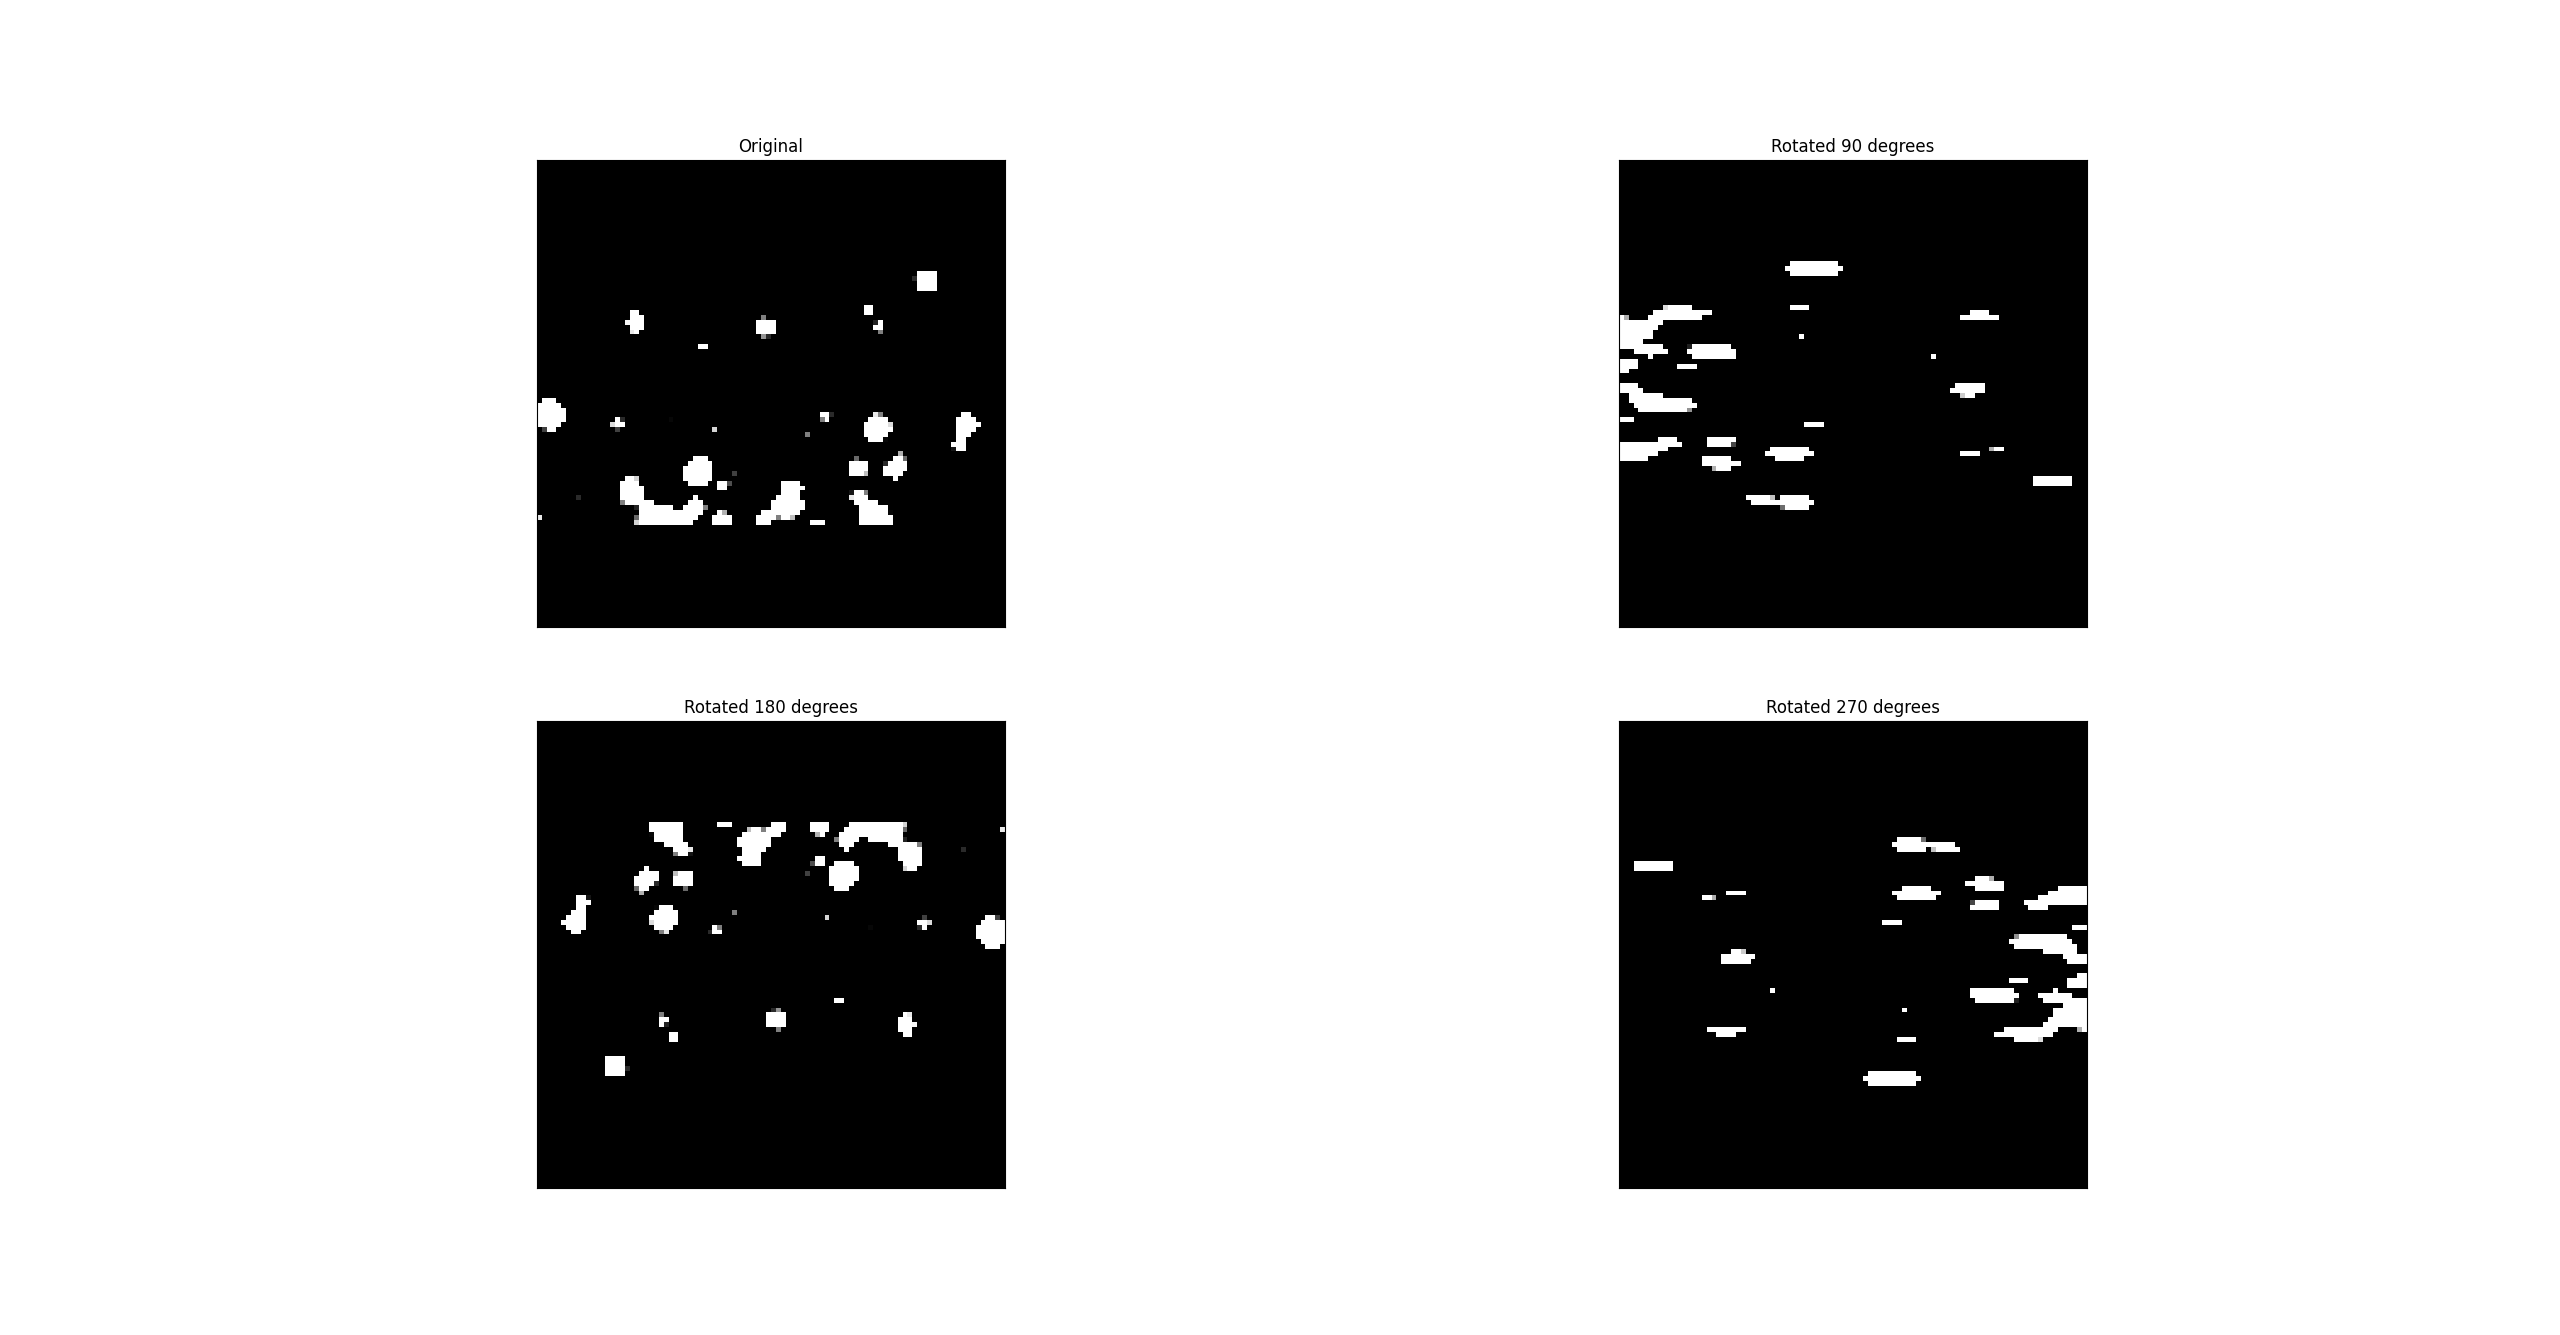
\includegraphics[width=.9\linewidth]{cnn_augmented_images}
   \caption{Example of augmented dataset for training the \acrlong{cnn}}
   \label{fig:cnn_aug_imgs}
\end{figure}

\section{Results}
\label{sec:results}

\begin{figure*}
  \centering
  \begin{subfigure}{.49\linewidth}
    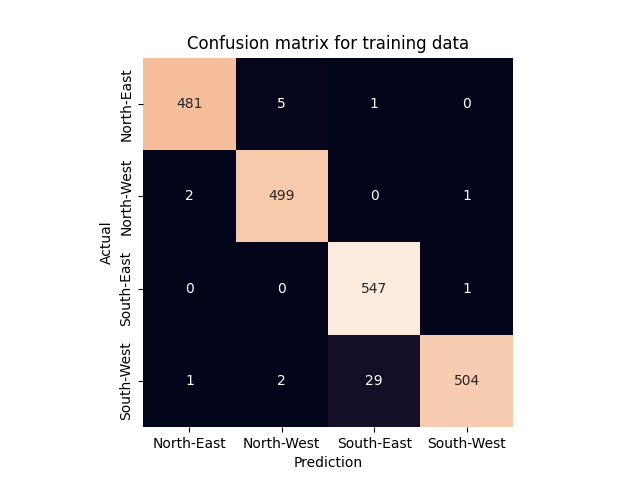
\includegraphics[width=\linewidth]{svm_cfsn_train}
    \caption{\acrshort{svm} confusion matrix for training data}
    \label{fig:svm_train}
  \end{subfigure}
  \hfill
  \begin{subfigure}{0.49\linewidth}
    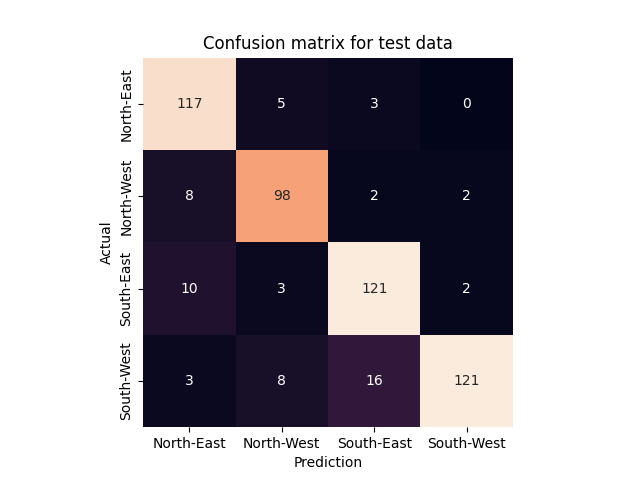
\includegraphics[width=\linewidth]{svm_cfsn_test}
    \caption{\acrshort{svm} confusion matrix for test data}
    \label{fig:svm_test}
  \end{subfigure}
  \caption{\acrlong{svm} classification results}
  \label{fig:svm_res}
\end{figure*}

\section{Conclusion}
\label{sec:conclusion}


%%%%%%%%% REFERENCES
{\small
\bibliographystyle{ieee_fullname}
\bibliography{egbib}
}

\end{document}
